\documentclass[10pt]{article}
\usepackage[utf8]{inputenc}
\usepackage[T1]{fontenc}
\usepackage{amsmath}
\usepackage{amsfonts}
\usepackage{amssymb}
\usepackage[version=4]{mhchem}
\usepackage{stmaryrd}
\usepackage{graphicx}
\usepackage[export]{adjustbox}
\graphicspath{ {./images/} }

%New command to display footnote whose markers will always be hidden
\let\svthefootnote\thefootnote
\newcommand\blfootnotetext[1]{%
  \let\thefootnote\relax\footnote{#1}%
  \addtocounter{footnote}{-1}%
  \let\thefootnote\svthefootnote%
}

%Overriding the \footnotetext command to hide the marker if its value is `0`
\let\svfootnotetext\footnotetext
\renewcommand\footnotetext[2][?]{%
  \if\relax#1\relax%
    \ifnum\value{footnote}=0\blfootnotetext{#2}\else\svfootnotetext{#2}\fi%
  \else%
    \if?#1\ifnum\value{footnote}=0\blfootnotetext{#2}\else\svfootnotetext{#2}\fi%
    \else\svfootnotetext[#1]{#2}\fi%
  \fi
}

\begin{document}
\section*{Bonds with exponentially decaying coupons}
Consider a bond issued at $t$ whose coupon at $t+j$ is $\rho^{j-1}$, with $\rho \in\left[0, \frac{1}{\beta}\right), \beta \in(0,1)$, and $j \in\{1,2, \ldots\} .^{1}$ Let $Q_{t, t-k}$ denote the price at $t$ of a bond issued at $t-k .{ }^{2}$ For $k=0$ we simply define $Q_{t} \equiv Q_{t, t}$. Hence, the flow of funds for a buyer of one unit of the bond at the time of issuance is:\\
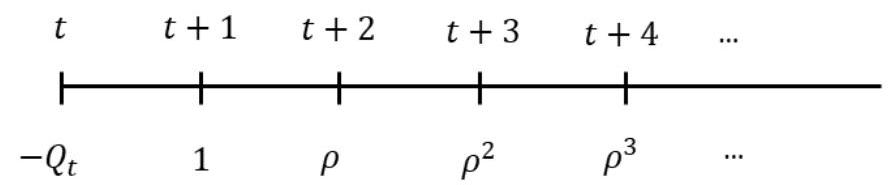
\includegraphics[max width=\textwidth, center]{2024_12_20_d3f1b1434ca90032aac2g-1(1)}

Compare the flow of funds, starting at $t$, for the following two strategies: (i) buy $\rho$ units of a bond issued at $t$; (ii) buy one unit of a bond issued at $t-1$. We have:\\
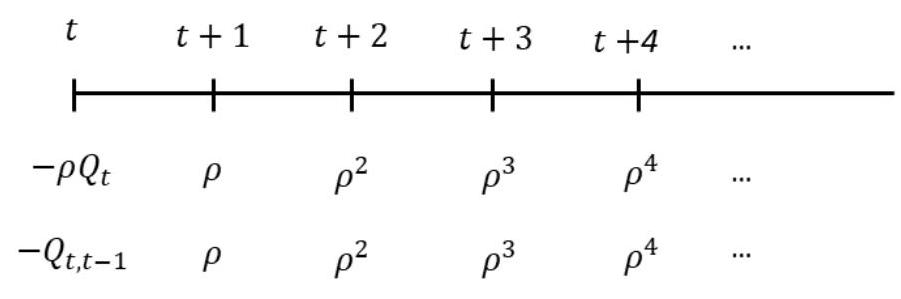
\includegraphics[max width=\textwidth, center]{2024_12_20_d3f1b1434ca90032aac2g-1(2)}

Since the flow of funds are exactly the same, no-arbitrage implies:

\begin{equation*}
Q_{t, t-1}=\rho Q_{t}
\end{equation*}

Now compare the flow of funds, starting at $t$, for the following three strategies: (i) buy $\rho^{2}$ units of a bond issued at $t$; (ii) buy $\rho$ units of a bond issued at $t-1$; (iii) buy one unit of a bond issued at $t-2$. We have:\\
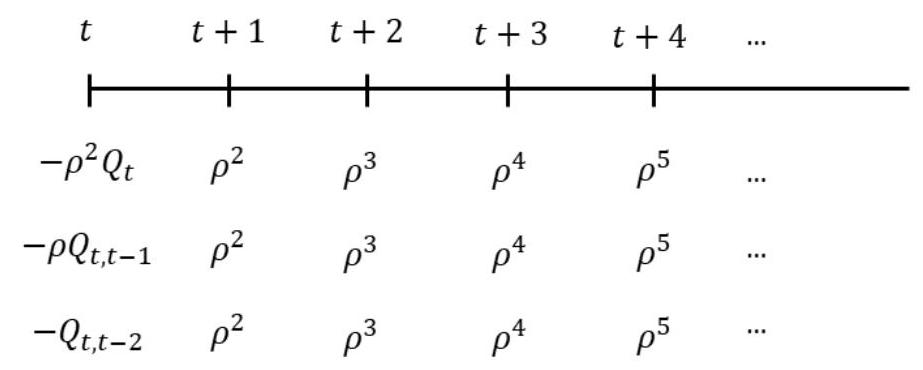
\includegraphics[max width=\textwidth, center]{2024_12_20_d3f1b1434ca90032aac2g-1}

Since the flow of funds are exactly the same, no-arbitrage implies: $Q_{t, t-2}=\rho Q_{t, t-1}=\rho^{2} Q_{t} \Rightarrow$

\begin{equation*}
Q_{t, t-2}=\rho^{2} Q_{t}
\end{equation*}

\footnotetext{${ }^{1}$ When $\rho=0$ and $k=1$ set $\rho^{k-1}=0^{0}=1$. As shown later, the constraint $\rho<\frac{1}{\beta}$ is included to ensure a well-defined duration in steady state.\\
${ }^{2} Q_{t+k, t}$ is the price at $t+k$, after the coupon at $t+k$ is paid.
}In general, for $k \in\{0,1,2, \ldots\}$ :

\begin{equation*}
Q_{t, t-k}=\rho^{k} Q_{t}
\end{equation*}

Suppose there's no uncertainty and consider the (net) nominal return between $t$ and $t+1$ of buying one unit of a bond issued at $t$ and selling it at $t+1$ (after collecting the coupon):

\begin{equation*}
\begin{aligned}
\text { Return }_{t, t+1} & =\frac{1+Q_{t+1, t}-Q_{t, t}}{Q_{t, t}} \\
& =\frac{1+\rho Q_{t+1}-Q_{t}}{Q_{t}} \\
& =\frac{1+\rho Q_{t+1}}{Q_{t}}-1
\end{aligned}
\end{equation*}

Suppose at $t$ you have access to a one-period risk-free bond with nominal return $i_{t}$. Then, no-arbitrage implies: Return $_{t, t+1}=i_{t} \Rightarrow$

\begin{equation*}
\frac{1+\rho Q_{t+1}}{Q_{t}}-1=i_{t}
\end{equation*}

Then:

\begin{equation*}
Q_{t}=\frac{1+\rho Q_{t+1}}{1+i_{t}}
\end{equation*}

Consider a steady state with constant nominal variables. The expression above implies: $Q=\frac{1+\rho Q}{1+i} \Rightarrow$ $Q(1+i)=1+\rho Q \Rightarrow Q(1+i-\rho)=1 \Rightarrow$

\begin{equation*}
Q=\frac{1}{1+i-\rho}
\end{equation*}

Yield to maturity\\
Let $y_{t}$ denote the yield to maturity at $t$ for a bond issued at $t$. Then, $y_{t}$ solves:

\begin{equation*}
Q_{t}=\frac{1}{1+y_{t}}+\frac{\rho}{\left(1+y_{t}\right)^{2}}+\frac{\rho^{2}}{\left(1+y_{t}\right)^{3}}+\frac{\rho^{3}}{\left(1+y_{t}\right)^{4}}+\ldots
\end{equation*}

Then:

\begin{equation*}
\begin{aligned}
& Q_{t}=\frac{1}{1+y_{t}}\left[1+\frac{\rho}{1+y_{t}}+\frac{\rho^{2}}{\left(1+y_{t}\right)^{2}}+\frac{\rho^{3}}{\left(1+y_{t}\right)^{3}}+\ldots\right] \\
& Q_{t}=\frac{1}{1+y_{t}}\left[1+\left(\frac{\rho}{1+y_{t}}\right)+\left(\frac{\rho}{1+y_{t}}\right)^{2}+\left(\frac{\rho}{1+y_{t}}\right)^{3}+\ldots\right] \\
& Q_{t}=\frac{1}{1+y_{t}} \frac{1}{1-\frac{\rho}{1+y_{t}}} \\
& Q_{t}=\frac{1}{1+y_{t}} \frac{1+y_{t}}{1+y_{t}-\rho} \\
& Q_{t}=\frac{1}{1+y_{t}-\rho}
\end{aligned}
\end{equation*}

Then: $1+y_{t}-\rho=\frac{1}{Q_{t}} \Rightarrow$

\begin{equation*}
y_{t}=\frac{1}{Q_{t}}+\rho-1
\end{equation*}

Consider a steady state with constant nominal varibles. Then:

\begin{equation*}
\begin{aligned}
& y=\frac{1}{Q}+\rho-1 \\
& y=\frac{1}{1+i-\rho}+\rho-1 \\
& y=1+i-\rho+\rho-1 \\
& y=i
\end{aligned}
\end{equation*}

\section*{Duration}
Let $D_{t}$ denote the duration at $t$ for a bond issued at $t$ :

\begin{equation*}
D_{t}=\sum_{\tau=1}^{\infty} \omega_{\tau} \tau
\end{equation*}

where $\omega_{\tau}=\frac{\frac{\rho^{\tau-1}}{\left(1+y_{t}\right)^{2}}}{Q_{t}}$, with $\sum_{\tau=1}^{\infty} \omega_{\tau}=1$. Then:

\begin{equation*}
\left.\left.\begin{array}{rl}
D_{t} & =\sum_{\tau=1}^{\infty} \frac{\rho^{\tau-1}}{Q_{t}\left(1+y_{t}\right)^{\tau}} \tau \\
D_{t} & =\frac{1}{Q_{t}\left(1+y_{t}\right)} \sum_{\tau=1}^{\infty} \tau\left(\frac{\rho}{1+y_{t}}\right)^{\tau-1} \\
D_{t} & =\frac{1}{Q_{t}\left(1+y_{t}\right)} \sum_{\tau=1}^{\infty} \tau \phi^{\tau-1} \quad \text { where } \phi \equiv \frac{\rho}{1+y_{t}} \\
D_{t} & =\frac{1}{Q_{t}\left(1+y_{t}\right)}\left[1+2 \phi+3 \phi^{2}+4 \phi^{3}+5 \phi^{4}+\ldots\right] \\
D_{t} & =\frac{1}{Q_{t}\left(1+y_{t}\right)}\left[1+\phi+\phi+\phi^{2}+\phi^{2}+\phi^{2}+\phi^{3}+\phi^{3}+\phi^{3}+\phi^{3}+\phi^{4}+\phi^{4}+\phi^{4}+\phi^{4}+\phi^{4}+\ldots\right] \\
D_{t} & =\frac{1}{Q_{t}\left(1+y_{t}\right)}\left[\left(\phi^{2}+\phi^{3}+\phi^{4}+\ldots\right)+\left(\phi^{3}+\phi^{4}+\ldots\right)+\left(\phi^{4}+\ldots\right)+\ldots\right.
\end{array}\right]\right]
\end{equation*}

Then:

\begin{equation*}
D_{t}=\frac{1+y_{t}}{1+y_{t}-\rho}
\end{equation*}

As expected, duration is a measure of the sensitivity of the price of the bond to its yield-to-maturity. Using $Q_{t}=\frac{1}{1+y_{t}-\rho}$ we can compute the elasticity of $Q_{t}$ with respect to $1+y_{t}$ :

\begin{equation*}
\begin{aligned}
& -\frac{1+y_{t}}{Q_{t}} \frac{\partial Q_{t}}{\partial\left(1+y_{t}\right)}=-\frac{1+y_{t}}{Q_{t}} \frac{-1}{\left(1+y_{t}-\rho\right)^{2}} \\
& -\frac{1+y_{t}}{Q_{t}} \frac{\partial Q_{t}}{\partial\left(1+y_{t}\right)}=\frac{1+y_{t}}{1+y_{t}-\rho} \frac{1}{\left(1+y_{t}-\rho\right)^{2}} \\
& -\frac{1+y_{t}}{Q_{t}} \frac{\partial Q_{t}}{\partial\left(1+y_{t}\right)}=\frac{1+y_{t}}{1+y_{t}-\rho} \\
& -\frac{1+y_{t}}{Q_{t}} \frac{\partial Q_{t}}{\partial\left(1+y_{t}\right)}=D_{t}
\end{aligned}
\end{equation*}

In a steady state with constant nominal variables we get: $D=\frac{1+y}{1+y-\rho}$. Using $y=i$ we get:

\begin{equation*}
\begin{aligned}
D & =\frac{1+i}{1+i-\rho} \\
D & =\frac{1}{1-\frac{\rho}{1+i}}
\end{aligned}
\end{equation*}

\section*{Budget constraint}
Budget constraint at $t$ :

\begin{equation*}
P_{t} c_{t}+\frac{b_{t+1}}{1+i_{t}}+Q_{t} b_{t+1}^{\rho}=P_{t} y_{t}+b_{t}+b_{t}^{\rho}+\rho b_{t-1}^{\rho}+\rho^{2} b_{t-2}^{\rho}+\ldots+\rho^{t-1} b_{1}^{\rho}+\rho^{t} b_{0}^{\rho}+\rho^{t+1} b_{-1}^{\rho}+\ldots
\end{equation*}

where $b_{t+1}$ denotes the quantity of one-period bonds bought at $t$, and $b_{t+1}^{\rho}$ is the quantity of long-period bonds bought at $t{ }^{3}$

Define:

\begin{equation*}
B_{t} \equiv b_{t}^{\rho}+\rho b_{t-1}^{\rho}+\rho^{2} b_{t-2}^{\rho}+\ldots+\rho^{t-1} b_{1}^{\rho}+\rho^{t} b_{0}^{\rho}+\rho^{t+1} b_{-1}^{\rho}+\ldots
\end{equation*}

Notice that:

\begin{equation*}
\begin{aligned}
& B_{t+1}=b_{t+1}^{\rho}+\rho b_{t}^{\rho}+\rho^{2} b_{t-1}^{\rho}+\ldots+\rho^{t} b_{1}^{\rho}+\rho^{t+1} b_{0}^{\rho}+\rho^{t+2} b_{-1}^{\rho}+\ldots \\
& B_{t+1}=b_{t+1}^{\rho}+\rho\left(b_{t}^{\rho}+\rho b_{t-1}^{\rho}+\ldots+\rho^{t-1} b_{1}^{\rho}+\rho^{t} b_{0}^{\rho}+\rho^{t+1} b_{-1}^{\rho}+\ldots\right) \\
& B_{t+1}=b_{t+1}^{\rho}+\rho B_{t}
\end{aligned}
\end{equation*}

Then:

\begin{equation*}
b_{t+1}^{\rho}=B_{t+1}-\rho B_{t}
\end{equation*}

\footnotetext{${ }^{3}$ We use the term long-period bonds to denote the bonds with exponentially decaying coupons.
}With this notation we can rewrite the budget constraint as follows:

\begin{equation*}
\begin{aligned}
& P_{t} c_{t}+\frac{b_{t+1}}{1+i_{t}}+Q_{t}\left(B_{t+1}-\rho B_{t}\right)=P_{t} y_{t}+b_{t}+B_{t} \\
& P_{t} c_{t}+\frac{b_{t+1}}{1+i_{t}}+Q_{t} B_{t+1}=P_{t} y_{t}+b_{t}+\left(1+\rho Q_{t}\right) B_{t}
\end{aligned}
\end{equation*}

Alternatively, we can think that in every period the agent sells the long-term bonds bought in the previous period (after collecting the coupons), and buys new long-term bonds. In this case, the budget constraint at $t$ is:

\begin{equation*}
P_{t} c_{t}+\frac{b_{t+1}}{1+i_{t}}+Q_{t} b_{t+1}^{\rho}=P_{t} y_{t}+b_{t}+b_{t}^{\rho}+Q_{t, t-1} b_{t}^{\rho}
\end{equation*}

Using $Q_{t, t-1}=\rho Q_{t}$ we get:

\begin{equation*}
\begin{gathered}
P_{t} c_{t}+\frac{b_{t+1}}{1+i_{t}}+Q_{t} b_{t+1}^{\rho}=P_{t} y_{t}+b_{t}+b_{t}^{\rho}+\rho Q_{t} b_{t}^{\rho} \\
P_{t} c_{t}+\frac{b_{t+1}}{1+i_{t}}+Q_{t} b_{t+1}^{\rho}=P_{t} y_{t}+b_{t}+\left(1+\rho Q_{t}\right) b_{t}^{\rho}
\end{gathered}
\end{equation*}

Notice that the two forms of the budget contraint have the same structure.

\section*{Utility maximization}
Using the second form of the budget constraint we have:

\begin{equation*}
\begin{array}{cl}
\max _{\left\{c_{t}, b_{t+1}, b_{t+1}^{\rho}\right\}_{t=0}^{\infty}} & \sum_{t=0}^{\infty} \beta^{t} u\left(c_{t}\right) \\
\text { s.t. } & P_{t} c_{t}+\frac{b_{t+1}}{1+i_{t}}+Q_{t} b_{t+1}^{\rho}=P_{t} y_{t}+b_{t}+\left(1+\rho Q_{t}\right) b_{t}^{\rho} \\
& b_{0}, b_{0}^{\rho} \text { given }
\end{array}
\end{equation*}

with appropriate No-Ponzi constraints.\\
Lagrangian:

\begin{equation*}
\mathcal{L}=\sum_{t=0}^{\infty} \beta^{t} u\left(c_{t}\right)+\sum_{t=0}^{\infty} \beta^{t} \lambda_{t}\left[P_{t} y_{t}+b_{t}+\left(1+\rho Q_{t}\right) b_{t}^{\rho}-P_{t} c_{t}-\frac{b_{t+1}}{1+i_{t}}-Q_{t} b_{t+1}^{\rho}\right]
\end{equation*}

FOC

\begin{equation*}
\begin{array}{ll}
c_{t}: & \beta^{t} u^{\prime}\left(c_{t}\right)=\beta^{t} \lambda_{t} P_{t} \\
b_{t+1}: & -\beta^{t} \lambda_{t} \frac{1}{1+i_{t}}+\beta^{t+1} \lambda_{t+1}=0 \\
b_{t+1}^{\rho}: & -\beta^{t} \lambda_{t} Q_{t}+\beta^{t+1} \lambda_{t+1}\left(1+\rho Q_{t+1}\right)=0
\end{array}
\end{equation*}

Then:

\begin{equation*}
\begin{aligned}
& \lambda_{t}=\frac{u^{\prime}\left(c_{t}\right)}{P_{t}} \\
& \lambda_{t}=\left(1+i_{t}\right) \beta \lambda_{t+1} \\
& \lambda_{t}=\frac{1+\rho Q_{t+1}}{Q_{t}} \beta \lambda_{t+1}
\end{aligned}
\end{equation*}

Combining $\lambda_{t}=\frac{u^{\prime}\left(c_{t}\right)}{P_{t}}$ and $\lambda_{t}=\left(1+i_{t}\right) \beta \lambda_{t+1}$ we get the standard Euler Equation:

\begin{equation*}
\begin{aligned}
& \frac{u^{\prime}\left(c_{t}\right)}{\beta u^{\prime}\left(c_{t+1}\right)}=\left(1+i_{t}\right) \frac{P_{t}}{P_{t+1}} \\
& \frac{u^{\prime}\left(c_{t}\right)}{\beta u^{\prime}\left(c_{t+1}\right)}=1+r_{t}
\end{aligned}
\end{equation*}

where $1+r_{t} \equiv\left(1+i_{t}\right) \frac{P_{t}}{P_{t+1}}$.\\
Combining $\lambda_{t}=\left(1+i_{t}\right) \beta \lambda_{t+1}$ and $\lambda_{t}=\frac{1+\rho Q_{t+1}}{Q_{t}} \beta \lambda_{t+1}$ we get the no-arbitrage condition we derived earlier:

\begin{equation*}
\frac{1+\rho Q_{t+1}}{Q_{t}}=1+i_{t}
\end{equation*}

Notice that without this condition the household could borrow at the lower return and lend at the higher one. But his would make the household's budget set unbounded, and the utility-maximization problem would have no solution (under the standard assumption that $u^{\prime}>0$ ).\\
Consider a steady state with constant real and nominal variables. From the Euler Equation we get: $\frac{u^{\prime}(c)}{\beta u^{\prime}(c)}=(1+i) \frac{P}{P} \Rightarrow$

\begin{equation*}
1+i=\frac{1}{\beta}
\end{equation*}

Substituting into $D=\frac{1}{1-\frac{\rho}{1+i}}$ we get the following expression for the duration of the bond:

\begin{equation*}
D=\frac{1}{1-\beta \rho}
\end{equation*}

Notice that the constraint $\rho<\frac{1}{\beta}$ implies that duration is positive.


\end{document}